\documentclass[man]{apa6}

\usepackage{amssymb,amsmath}
\usepackage{ifxetex,ifluatex}
\usepackage{fixltx2e} % provides \textsubscript
\ifnum 0\ifxetex 1\fi\ifluatex 1\fi=0 % if pdftex
  \usepackage[T1]{fontenc}
  \usepackage[utf8]{inputenc}
\else % if luatex or xelatex
  \ifxetex
    \usepackage{mathspec}
    \usepackage{xltxtra,xunicode}
  \else
    \usepackage{fontspec}
  \fi
  \defaultfontfeatures{Mapping=tex-text,Scale=MatchLowercase}
  \newcommand{\euro}{€}
\fi
% use upquote if available, for straight quotes in verbatim environments
\IfFileExists{upquote.sty}{\usepackage{upquote}}{}
% use microtype if available
\IfFileExists{microtype.sty}{\usepackage{microtype}}{}

% Table formatting
\usepackage{longtable, booktabs}
\usepackage{lscape}
% \usepackage[counterclockwise]{rotating}   % Landscape page setup for large tables
\usepackage{multirow}		% Table styling
\usepackage{tabularx}		% Control Column width
\usepackage[flushleft]{threeparttable}	% Allows for three part tables with a specified notes section
\usepackage{threeparttablex}            % Lets threeparttable work with longtable

% Create new environments so endfloat can handle them
% \newenvironment{ltable}
%   {\begin{landscape}\begin{center}\begin{threeparttable}}
%   {\end{threeparttable}\end{center}\end{landscape}}

\newenvironment{lltable}
  {\begin{landscape}\begin{center}\begin{ThreePartTable}}
  {\end{ThreePartTable}\end{center}\end{landscape}}

  \usepackage{ifthen} % Only add declarations when endfloat package is loaded
  \ifthenelse{\equal{\string man}{\string man}}{%
   \DeclareDelayedFloatFlavor{ThreePartTable}{table} % Make endfloat play with longtable
   % \DeclareDelayedFloatFlavor{ltable}{table} % Make endfloat play with lscape
   \DeclareDelayedFloatFlavor{lltable}{table} % Make endfloat play with lscape & longtable
  }{}%



% The following enables adjusting longtable caption width to table width
% Solution found at http://golatex.de/longtable-mit-caption-so-breit-wie-die-tabelle-t15767.html
\makeatletter
\newcommand\LastLTentrywidth{1em}
\newlength\longtablewidth
\setlength{\longtablewidth}{1in}
\newcommand\getlongtablewidth{%
 \begingroup
  \ifcsname LT@\roman{LT@tables}\endcsname
  \global\longtablewidth=0pt
  \renewcommand\LT@entry[2]{\global\advance\longtablewidth by ##2\relax\gdef\LastLTentrywidth{##2}}%
  \@nameuse{LT@\roman{LT@tables}}%
  \fi
\endgroup}


  \usepackage{graphicx}
  \makeatletter
  \def\maxwidth{\ifdim\Gin@nat@width>\linewidth\linewidth\else\Gin@nat@width\fi}
  \def\maxheight{\ifdim\Gin@nat@height>\textheight\textheight\else\Gin@nat@height\fi}
  \makeatother
  % Scale images if necessary, so that they will not overflow the page
  % margins by default, and it is still possible to overwrite the defaults
  % using explicit options in \includegraphics[width, height, ...]{}
  \setkeys{Gin}{width=\maxwidth,height=\maxheight,keepaspectratio}
\ifxetex
  \usepackage[setpagesize=false, % page size defined by xetex
              unicode=false, % unicode breaks when used with xetex
              xetex]{hyperref}
\else
  \usepackage[unicode=true]{hyperref}
\fi
\hypersetup{breaklinks=true,
            pdfauthor={},
            pdftitle={Assignment Statistics 5},
            colorlinks=true,
            citecolor=blue,
            urlcolor=blue,
            linkcolor=black,
            pdfborder={0 0 0}}
\urlstyle{same}  % don't use monospace font for urls

\setlength{\parindent}{0pt}
%\setlength{\parskip}{0pt plus 0pt minus 0pt}

\setlength{\emergencystretch}{3em}  % prevent overfull lines


% Manuscript styling
\captionsetup{font=singlespacing,justification=justified}
\usepackage{csquotes}
\usepackage{upgreek}



\usepackage{tikz} % Variable definition to generate author note

% fix for \tightlist problem in pandoc 1.14
\providecommand{\tightlist}{%
  \setlength{\itemsep}{0pt}\setlength{\parskip}{0pt}}

% Essential manuscript parts
  \title{Assignment Statistics 5}

  \shorttitle{Bayesian hierarchical modeling}


  \author{Gustavo Villca Ponce\textsuperscript{1}, MohammadHossein Haqiqatkhah\textsuperscript{2}, Sigert Ariens\textsuperscript{3}, \& Bavo Kempen\textsuperscript{4}}

  % \def\affdep{{"", "", "", ""}}%
  % \def\affcity{{"", "", "", ""}}%

  \affiliation{
    \vspace{0.5cm}
          \textsuperscript{1} r0292033\\
          \textsuperscript{2} r0607671\\
          \textsuperscript{3} r0446864\\
          \textsuperscript{4} r0585283\\
          \textsuperscript{} Faculty of Psychology and Educational Sciences, KU Leuven.  }



      \keywords{\\

      \indent  1613
    }
  




\usepackage{amsthm}
\newtheorem{theorem}{Theorem}[section]
\newtheorem{lemma}{Lemma}[section]
\theoremstyle{definition}
\newtheorem{definition}{Definition}[section]
\newtheorem{corollary}{Corollary}[section]
\newtheorem{proposition}{Proposition}[section]
\theoremstyle{definition}
\newtheorem{example}{Example}[section]
\theoremstyle{definition}
\newtheorem{exercise}{Exercise}[section]
\theoremstyle{remark}
\newtheorem*{remark}{Remark}
\newtheorem*{solution}{Solution}
\begin{document}

\maketitle

\setcounter{secnumdepth}{0}



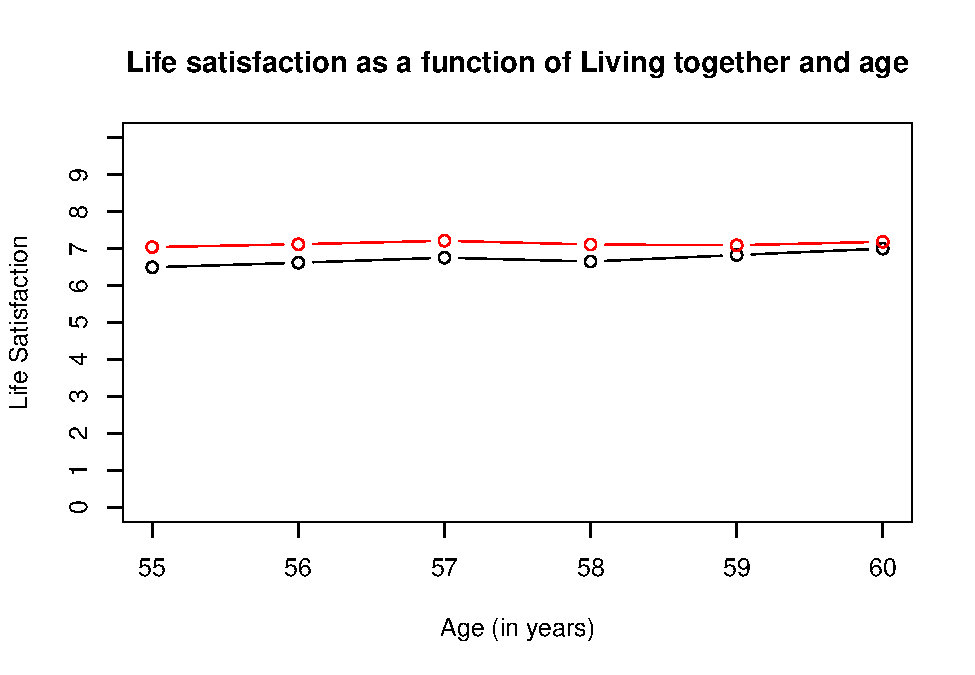
\includegraphics{Statistics-5-report-final-hours_files/figure-latex/exploratory plots-1.pdf}
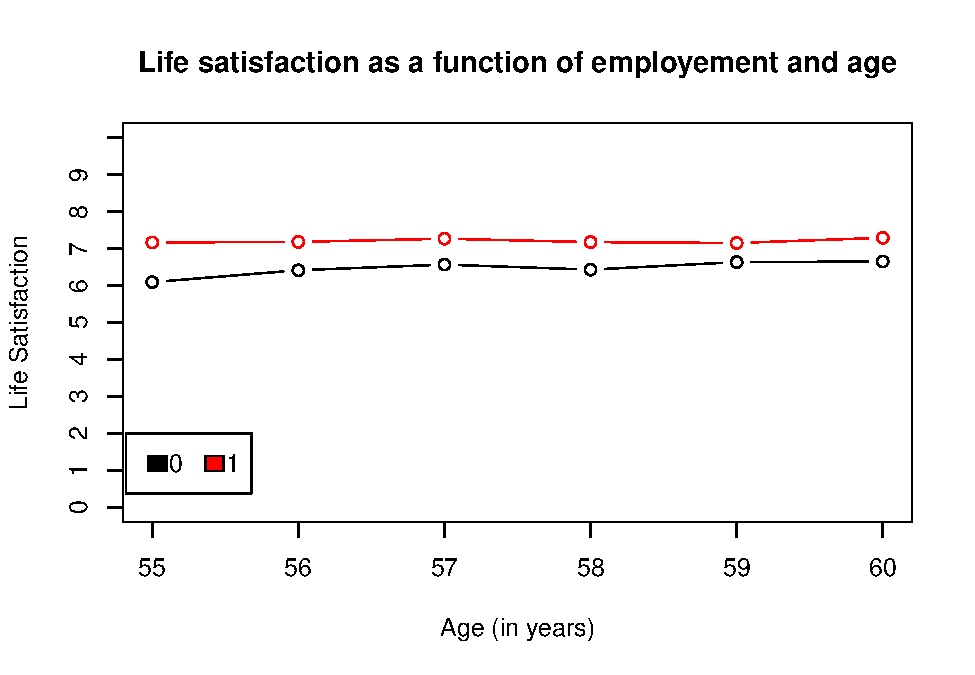
\includegraphics{Statistics-5-report-final-hours_files/figure-latex/exploratory plots-2.pdf}
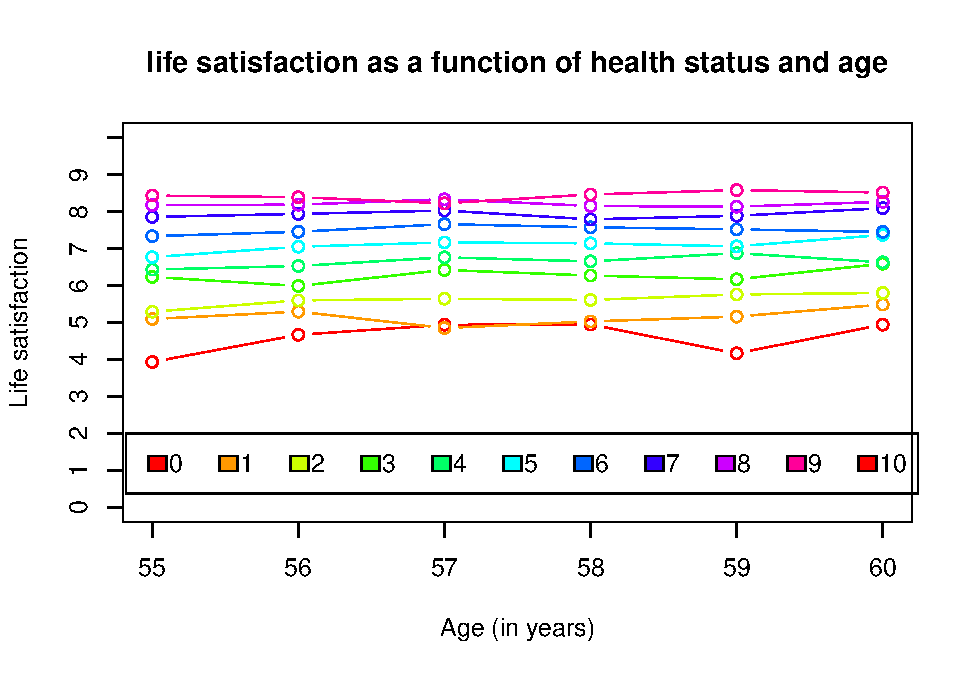
\includegraphics{Statistics-5-report-final-hours_files/figure-latex/exploratory plots-3.pdf}

\begin{lltable}
\begin{TableNotes}[para]
\textit{Note.} Full model.
\end{TableNotes}
\small{
\begin{longtable}{llllllllllll}\noalign{\getlongtablewidth\global\LTcapwidth=\longtablewidth}
\caption{\label{tab:tables of summaries}The first model}\\
\toprule
 & \multicolumn{1}{c}{Lower95} & \multicolumn{1}{c}{Median} & \multicolumn{1}{c}{Upper95} & \multicolumn{1}{c}{Mean} & \multicolumn{1}{c}{SD} & \multicolumn{1}{c}{Mode} & \multicolumn{1}{c}{MCerr} & \multicolumn{1}{c}{MC\%ofSD} & \multicolumn{1}{c}{SSeff} & \multicolumn{1}{c}{AC.1800} & \multicolumn{1}{c}{psrf}\\
\midrule
ss[1] & 0.54 & 0.60 & 0.66 & 0.60 & 0.03 & 0.60 & 0.00 & 2.20 & 2,000.00 & -0.01 & 1.00\\
ss[2] & 0.26 & 0.29 & 0.32 & 0.29 & 0.02 & 0.29 & 0.00 & 2.20 & 2,000.00 & 0.02 & 1.00\\
ss[3] & 0.42 & 0.57 & 0.72 & 0.57 & 0.08 & 0.56 & 0.00 & 2.20 & 2,000.00 & -0.02 & 1.00\\
cor12 & -0.02 & -0.01 & 0.01 & -0.01 & 0.01 & -0.01 & 0.00 & 2.10 & 2,363.00 & -0.01 & 1.00\\
cor13 & -0.36 & -0.21 & -0.08 & -0.22 & 0.08 & -0.20 & 0.00 & 2.20 & 2,000.00 & -0.02 & 1.00\\
cor23 & -0.15 & -0.07 & 0.00 & -0.07 & 0.04 & -0.06 & 0.00 & 2.20 & 2,000.00 & -0.03 & 1.00\\
betamu[1] & -0.39 & -0.30 & -0.21 & -0.30 & 0.05 & -0.29 & 0.00 & 2.00 & 2,551.00 & 0.00 & 1.00\\
betamu[2] & 0.30 & 0.35 & 0.40 & 0.35 & 0.03 & 0.35 & 0.00 & 2.20 & 2,106.00 & -0.02 & 1.00\\
betamu[3] & 0.11 & 0.19 & 0.27 & 0.19 & 0.04 & 0.19 & 0.00 & 2.20 & 2,060.00 & 0.01 & 1.00\\
betax[1] & 0.13 & 0.21 & 0.29 & 0.21 & 0.04 & 0.21 & 0.00 & 2.30 & 1,880.00 & -0.02 & 1.00\\
betax[2] & -0.03 & -0.02 & 0.00 & -0.02 & 0.01 & -0.02 & 0.00 & 2.20 & 2,000.00 & 0.04 & 1.00\\
betax[3] & -0.04 & -0.01 & 0.03 & -0.01 & 0.02 & -0.01 & 0.00 & 2.20 & 2,098.00 & 0.00 & 1.00\\
betax[4] & -0.02 & 0.02 & 0.05 & 0.02 & 0.02 & 0.02 & 0.00 & 2.30 & 1,903.00 & 0.02 & 1.00\\
betax[5] & 0.01 & 0.07 & 0.14 & 0.08 & 0.03 & 0.08 & 0.00 & 2.20 & 2,000.00 & -0.01 & 1.00\\
\bottomrule
\addlinespace
\insertTableNotes
\end{longtable}
}
\end{lltable}

\begin{lltable}
\begin{TableNotes}[para]
\textit{Note.} Reduced model.
\end{TableNotes}
\small{
\begin{longtable}{llllllllllll}\noalign{\getlongtablewidth\global\LTcapwidth=\longtablewidth}
\caption{\label{tab:tables of summaries}The Second model}\\
\toprule
 & \multicolumn{1}{c}{Lower95} & \multicolumn{1}{c}{Median} & \multicolumn{1}{c}{Upper95} & \multicolumn{1}{c}{Mean} & \multicolumn{1}{c}{SD} & \multicolumn{1}{c}{Mode} & \multicolumn{1}{c}{MCerr} & \multicolumn{1}{c}{MC\%ofSD} & \multicolumn{1}{c}{SSeff} & \multicolumn{1}{c}{AC.2000} & \multicolumn{1}{c}{psrf}\\
\midrule
ss[1] & 0.58 & 0.65 & 0.74 & 0.66 & 0.04 & 0.65 & 0.00 & 1.70 & 3,650.00 & 0.01 & 1.00\\
ss[2] & 0.42 & 0.61 & 0.78 & 0.61 & 0.09 & 0.60 & 0.00 & 1.70 & 3,452.00 & 0.01 & 1.00\\
cor12 & -0.46 & -0.24 & -0.09 & -0.25 & 0.10 & -0.23 & 0.00 & 1.70 & 3,421.00 & 0.01 & 1.00\\
betamu[1] & -0.35 & -0.24 & -0.13 & -0.24 & 0.06 & -0.24 & 0.00 & 1.60 & 4,000.00 & -0.04 & 1.00\\
betamu[2] & 0.07 & 0.18 & 0.28 & 0.18 & 0.05 & 0.18 & 0.00 & 1.60 & 3,787.00 & -0.01 & 1.00\\
betax[1] & 0.08 & 0.19 & 0.29 & 0.19 & 0.05 & 0.20 & 0.00 & 1.60 & 4,000.00 & -0.03 & 1.00\\
betax[2] & -0.01 & 0.01 & 0.02 & 0.01 & 0.01 & 0.01 & 0.00 & 1.70 & 3,441.00 & -0.01 & 1.00\\
sigma & 0.59 & 0.61 & 0.62 & 0.61 & 0.01 & 0.61 & 0.00 & 1.60 & 4,000.00 & 0.00 & 1.00\\
\bottomrule
\addlinespace
\insertTableNotes
\end{longtable}
}
\end{lltable}

\begin{lltable}
\begin{TableNotes}[para]
\textit{Note.} Sensitivity analysis 1.
\end{TableNotes}
\small{
\begin{longtable}{llllllllllll}\noalign{\getlongtablewidth\global\LTcapwidth=\longtablewidth}
\caption{\label{tab:tables of summaries}Sensitivity 1}\\
\toprule
 & \multicolumn{1}{c}{Lower95} & \multicolumn{1}{c}{Median} & \multicolumn{1}{c}{Upper95} & \multicolumn{1}{c}{Mean} & \multicolumn{1}{c}{SD} & \multicolumn{1}{c}{Mode} & \multicolumn{1}{c}{MCerr} & \multicolumn{1}{c}{MC\%ofSD} & \multicolumn{1}{c}{SSeff} & \multicolumn{1}{c}{AC.1500} & \multicolumn{1}{c}{psrf}\\
\midrule
ss[1] & 0.54 & 0.60 & 0.66 & 0.60 & 0.03 & 0.60 & 0.00 & 2.30 & 1,879.00 & -0.04 & 1.00\\
ss[2] & 0.26 & 0.29 & 0.32 & 0.29 & 0.02 & 0.28 & 0.00 & 2.30 & 1,905.00 & 0.00 & 1.00\\
ss[3] & 0.42 & 0.57 & 0.73 & 0.57 & 0.08 & 0.58 & 0.00 & 2.20 & 2,116.00 & 0.00 & 1.00\\
cor12 & -0.02 & -0.01 & 0.01 & -0.01 & 0.01 & -0.01 & 0.00 & 2.20 & 2,000.00 & 0.01 & 1.00\\
cor13 & -0.36 & -0.21 & -0.08 & -0.22 & 0.08 & -0.20 & 0.00 & 2.20 & 2,070.00 & 0.00 & 1.00\\
cor23 & -0.16 & -0.07 & 0.00 & -0.07 & 0.04 & -0.07 & 0.00 & 2.10 & 2,309.00 & -0.01 & 1.00\\
betamu[1] & -0.39 & -0.30 & -0.22 & -0.30 & 0.05 & -0.30 & 0.00 & 2.30 & 1,875.00 & -0.02 & 1.00\\
betamu[2] & 0.29 & 0.35 & 0.40 & 0.35 & 0.03 & 0.35 & 0.00 & 2.10 & 2,178.00 & -0.02 & 1.00\\
betamu[3] & 0.10 & 0.18 & 0.27 & 0.18 & 0.04 & 0.18 & 0.00 & 2.20 & 2,000.00 & 0.02 & 1.00\\
betax[1] & 0.13 & 0.21 & 0.29 & 0.21 & 0.04 & 0.22 & 0.00 & 2.20 & 2,150.00 & 0.02 & 1.00\\
betax[2] & 0.01 & 0.08 & 0.14 & 0.07 & 0.03 & 0.07 & 0.00 & 2.10 & 2,271.00 & 0.00 & 1.00\\
betax[3] & -0.04 & -0.01 & 0.03 & -0.01 & 0.02 & -0.01 & 0.00 & 2.20 & 2,000.00 & 0.01 & 1.00\\
betax[4] & -0.03 & -0.02 & 0.00 & -0.02 & 0.01 & -0.02 & 0.00 & 2.20 & 2,000.00 & 0.01 & 1.00\\
betax[5] & -0.01 & 0.02 & 0.06 & 0.02 & 0.02 & 0.02 & 0.00 & 2.20 & 2,000.00 & 0.00 & 1.00\\
betax[6] & -0.01 & 0.00 & 0.01 & 0.00 & 0.01 & 0.00 & 0.00 & 2.30 & 1,945.00 & 0.00 & 1.00\\
sigma & 0.59 & 0.60 & 0.62 & 0.60 & 0.01 & 0.60 & 0.00 & 2.20 & 2,000.00 & 0.01 & 1.00\\
\bottomrule
\addlinespace
\insertTableNotes
\end{longtable}
}
\end{lltable}

\begin{lltable}
\begin{TableNotes}[para]
\textit{Note.} Sensitivity analysis 2.
\end{TableNotes}
\small{
\begin{longtable}{llllllllllll}\noalign{\getlongtablewidth\global\LTcapwidth=\longtablewidth}
\caption{\label{tab:tables of summaries}Sensitivity 2}\\
\toprule
 & \multicolumn{1}{c}{Lower95} & \multicolumn{1}{c}{Median} & \multicolumn{1}{c}{Upper95} & \multicolumn{1}{c}{Mean} & \multicolumn{1}{c}{SD} & \multicolumn{1}{c}{Mode} & \multicolumn{1}{c}{MCerr} & \multicolumn{1}{c}{MC\%ofSD} & \multicolumn{1}{c}{SSeff} & \multicolumn{1}{c}{AC.3000} & \multicolumn{1}{c}{psrf}\\
\midrule
ss[1] & 0.57 & 0.66 & 0.73 & 0.66 & 0.04 & 0.66 & 0.00 & 2.50 & 1,600.00 & 0.02 & 1.01\\
ss[2] & 0.42 & 0.61 & 0.78 & 0.61 & 0.09 & 0.61 & 0.00 & 2.50 & 1,600.00 & 0.00 & 1.00\\
cor12 & -0.44 & -0.25 & -0.09 & -0.26 & 0.10 & -0.22 & 0.00 & 2.50 & 1,600.00 & 0.00 & 1.00\\
betamu[1] & -0.34 & -0.25 & -0.13 & -0.25 & 0.06 & -0.26 & 0.00 & 2.40 & 1,748.00 & 0.03 & 1.00\\
betamu[2] & 0.08 & 0.18 & 0.28 & 0.18 & 0.05 & 0.18 & 0.00 & 2.50 & 1,600.00 & 0.04 & 1.00\\
betax[1] & 0.09 & 0.20 & 0.29 & 0.20 & 0.05 & 0.20 & 0.00 & 2.50 & 1,644.00 & -0.02 & 1.00\\
betax[2] & -0.01 & 0.01 & 0.02 & 0.01 & 0.01 & 0.01 & 0.00 & 2.50 & 1,600.00 & 0.00 & 1.00\\
sigma & 0.59 & 0.60 & 0.62 & 0.60 & 0.01 & 0.60 & 0.00 & 2.50 & 1,600.00 & -0.04 & 1.01\\
rand & -9.23 & -0.04 & 8.79 & -0.03 & 4.96 & 0.10 & 0.12 & 2.40 & 1,710.00 & 0.01 & 1.00\\
rand2 & -9.12 & 0.14 & 9.11 & 0.06 & 5.41 & 0.48 & 0.14 & 2.50 & 1,600.00 & 0.01 & 1.00\\
\bottomrule
\addlinespace
\insertTableNotes
\end{longtable}
}
\end{lltable}

\hypertarget{research-question}{%
\section{Research question}\label{research-question}}

We explored the question of which factors are associated with life
satisfaction in the german sample of \$n=\$1236 using bayesian
regression techniques. Preceding the analysis, we omitted all missing
values, and standardized all non-binary variables. We centered age for
MCMC considerations. We also aimed to investigate whether we could
construct a model that could examine whether living together has an
effect on life satisfaction, when taking into account individual
differences, as posited by Lucas, Clark, Georgellis, and Diener (2003).
To this extent, we assured that this variable could interact with other
variables of intrest, and correlated with baseline individual
differences.

\hypertarget{method}{%
\section{Method}\label{method}}

We constructed a complex bayesian hierarchical regression model, with
life satisfaction as dependent variable, henceforth termed \(y_{i}\) and
then proceeded to construct a more simple model based on the exploratory
conclusions from the first. Our first model took into account the
variables of health satisfaction, living together, and employment status
as a between subjects factor, henceforth termed \(x_{2i}\), \(x_{3i}\),
and \(x_{4i}\) respectively. Age was included as \(x_{1i}\). We included
interactions between age and health satisfaction, age and partner, age
and employment, and health and employment. The choices of these
interactions were motivated by the fact that the \enquote{age} variable
changes equally for each individual, and interactions between this
variable and the others seemed most likely to influence life
satisfaction. Our final interaction was motivated by the idea that the
association of these variables could manifest its self in concrete
outcomes pertaining to work and health combinations. We used JAGS to
provide us with samples from the posterior.

In all our models, we assumed
\({y_{i}}\)\textasciitilde{}\({N(µ_{yi},\sigma)}\)

with \(\sigma\) \textasciitilde{} \({U(0.1, 1)}\)

\hypertarget{model-1}{%
\subsection{model 1}\label{model-1}}

\({µ_{yi} = \beta_{0i} + \beta_{2i}x_{2i} + \beta_{3i}x_{3i} +\beta_{4}x_{4i} + \beta_{5}x_{1i}x_{2i} + \beta_{6}x_{1i}x_{3i} + \beta_{6}x_{1i}x_{4i}+\beta_{7}x_{2i}x_{4i} }\)

\({\beta_{0i}}\) to \({\beta_{3i}}\) \textasciitilde{}
\({ N(\beta_{µ} , M ) }\)

and \({\beta_{µ}}\) \textasciitilde{} \({N(0, 0.0001)}\)

and \({M}\) \textasciitilde{} \({wish(1,4)}\)

With the between subjects and interactions \(\beta\)'s distributed as
\({N(0, \frac {1}{10^5})}\)

\hypertarget{model-2}{%
\subsection{model 2}\label{model-2}}

\({µ_{yi} = \beta_{0i} + \beta_{2i}x_{2i} + \beta_{3i}x_{3i} +\beta_{4}x_{4i} + \beta_{5}x_{1i}x_{2i}x_{4i}}\)

with \({\beta_{0i}}\) and \({\beta_{3i}}\) \textasciitilde{}
\({ N(\beta_{µ} , M ) }\)

and \({\beta_{µ}}\) \textasciitilde{} \({N(0, 0.0001)}\).

our non-correlating \(\beta_{2}\) and the between subjects and
interactions \(\beta\)'s \textasciitilde{} \({N(0, \frac {1}{10^5})}\).

\({y_{i} = \beta_{0i} + \beta_{2i}x_{2} + \beta_{3i}x_{3} +\beta_{4}x_{4} + \beta_{5}x_{1}x_{2} + \beta_{6}x_{1}x_{3} + \beta_{7}x_{1}x_{4}+\beta_{8}x_{2}x_{4} }\)

\hypertarget{exploring-the-data}{%
\section{Exploring the data}\label{exploring-the-data}}

We found that age could best be conceptualised as a factor interacting
with our other variables. Therefore, We plotted life satisfaction as a
function of living together and age, with living together is 1 and not
living together 0 (see Figure 1), life satisfaction as a function of
employment and age, with full time employed as 1 and partially -or, not
employed as 0 (see Figure 2) and life satisfaction as a function health
status and age with perceived health status ranging from 0-10 (see
Figure 3).

\hypertarget{jags-specifics}{%
\section{JAGS specifics}\label{jags-specifics}}

In order to assure convergence, we used a burn-in of 1000. We used 2000
iterations of the MCMC to assess the key models. For the first model, we
set a thinning value of 180 to assure no autocorrelation in the
sampling. For the second model, a thinning value of 200 was used. These
values were based on autocorrelation plots of exploratory runs of both
models.

\hypertarget{comparing-the-models-using-the-deviance-information-criterion-dic}{%
\section{Comparing the models using the Deviance Information Criterion
(DIC)}\label{comparing-the-models-using-the-deviance-information-criterion-dic}}

To compare the trade off between complexity and data description of our
models, we used the deviance information criterion (DIC). From the
analysis we obtained DIC values of `r dic.1.main´ and ´r dic.2.main´ for
the first and second model respectively. We can interprete this as
following" the model with the lowest DIC value is the model with the
smallest trade-off which in this case is our first model.

\hypertarget{sensitivity-analysis-of-the-models}{%
\section{Sensitivity analysis of the
models}\label{sensitivity-analysis-of-the-models}}

To assess whether our models were robust against choices of our pirors,
we fully randomised the means of the priors of the distributions from
which our parameters were sampled, using random uniform distributions
between -5 and 5. We also reduced the broadness of our precision and
variance parameters, from \(\frac {1}{10^5}\) to \(\frac {1}{10^2}\). We
found that these adaptations caused no interesting differences in our
models posterior. The results of these analyses can be found in table 3
and table 4. The difference in DIC criterium between the first model and
it's sensitiviy analysis was neligable(2.23and 2.23). For our second,
less complex model, the DICs were also comparable (2.45 and
2.45).Furthermore, the trend in which our first model obtained the
lowest DIC can also be found in the sensitivity analysis models (2.23
and 2.45).

\hypertarget{discussion}{%
\section{Discussion}\label{discussion}}

Since our DIC test suggested the more complex model to provide a better
trade-off between model complexity and data description, we decided to
use this model to interpret how life satisfaction changes according to
changes in other variables over time for different individuals. Since
the SSEFF of the components are quite similar, it is easy to interpret
the findings shown in Table 1. We found that our main effect variable of
\(\beta_{2i}\) pertaining to health satisfaction was indeed important in
describing differences in life satisfaction. Interestingly, the
\(\beta_{4i}\) pertaining to employment status demosntrated a positive
relationship between being employed at this age, and life satisfaction.
This too was in accordance with our exploratory analysis of the data. An
interaction plot between age, employment, and life satisfaction given
our models prediction can be found in Figure 4. While Lucas, Clark,
Georgellis, \& Diener (2003) reported that on average, living together
did not seem to have an effect on life satisfaction, we did find that
our \(\beta_{3i}\) value had a mean (\(M_{\beta_{3i}} = 0.19\)) and a
standard deviation (\(SD_{\beta_{3i}} = .04\)), indicating an influence.
However, the authors also noted that there were large individual
differences in this group. By allowing individual differences in this
variable, we may have captured it's effect more accurately. Furthermore,
The only relatively large correlation we found between our
within-subject variables was between \(\beta_{0i}\) and \(\beta_{3i}\),
indicting that living together is correlated with other baseline
individual differnces in the data. This does to some extent confirm the
conclusions of Lucas et al. (2003), although we did not test this
assumption directly.

\newpage

\hypertarget{references}{%
\section{References}\label{references}}

\begingroup
\setlength{\parindent}{-0.5in}
\setlength{\leftskip}{0.5in}

\hypertarget{refs}{}
\leavevmode\hypertarget{ref-lucas2003reexamining}{}%
Lucas, R. E., Clark, A. E., Georgellis, Y., \& Diener, E. (2003).
Reexamining adaptation and the set point model of happiness: Reactions
to changes in marital status. \emph{Journal of Personality and Social
Psychology}, \emph{84}(3), 527.

\endgroup






\end{document}
